\chapter{Historische Genauigkeit und Rechenkosten}
\index{Benchmark}\index{Rechenkosten}
\section{Messbestand und Umgebung}
Der versionierte Bestand
\path{benchmarks/baselines/m7-37c-linux-arm64.json} enthält 72 Läufe vom
28. September 2026: zwei Fälle, zwei direkte Backends, zwei Elementordnungen,
drei Netzgrößen und jeweils drei Wiederholungen. Daraus entstehen 24 Gruppen.
Der historische Quellcommit ist
\path{98ca442fe8954dcac15316cd1367f2b7819a21ab}.
Die Originaldatei wird bytegleich in das Handbucharchiv übernommen; aktuelle
Dokumentationsänderungen überschreiben diese Messungen nicht.

Die Umgebung war Docker/Linux auf aarch64 auf einem Apple M4, mit zehn
zugewiesenen logischen CPUs und 8\,217\,059\,328 Byte Container-RAM.
Verwendet wurden Python 3.12.3, NumPy 1.26.4, SciPy 1.14.1 und
PETSc 3.19.6 mit reellen 64-Bit-Skalaren, KSP \texttt{preonly} und PC
\texttt{lu}. Die sechs dokumentierten Thread-Umgebungsvariablen wurden auf 1
gesetzt; das ist eine angeforderte Begrenzung, keine Messung tatsächlich
aktiver Threads. Vollständige Bibliotheks-/BLAS-Angaben bleiben im JSON erhalten.

\section{Probleme und Messdefinition}
Die Netze mit $N=2,4,6$ zerlegen jeden Würfel in sechs Tetraeder; Tet10 erhält
gemeinsame Kantenmittelpunkte. Die Wärmequelle folgt aus
\begin{equation}
 T=1+x^4+\tfrac12y^4+\tfrac14z^4,\qquad
 k=1,\qquad Q=-12(x^2+\tfrac12y^2+\tfrac14z^2).
\end{equation}
Der synthetische Biegungsfall verwendet $E=100$, $\nu=0$, $a=0.01$ und
\begin{equation}
 \mathbf u=(-3ax^2z,0,ax^3)^\mathsf T,\qquad
 \mathbf b=(6Eaz,0,0)^\mathsf T.
\end{equation}
Beide Fälle sind analytisch hergestellte Lösungen, keine vermessenen Bauteile.
Insbesondere ist der Biegungsfall kein realer Kragarmversuch.

Die Zeit umfasst den ersten Solveraufruf einschließlich Randbedingungen,
Materialverarbeitung, Assembly, Faktorisierung, Nachverarbeitung und Provenienz.
Netzerzeugung, Imports, Backendinitialisierung, Export und unabhängige
Fehlerquadratur sind ausgeschlossen. RSS ist das Prozessmaximum seit
Prozessstart einschließlich Imports; es ist kein zusätzlicher Speicherbedarf
einer einzelnen Assembly. Der relative $H^1$-Halbnormfehler wird mit der
unabhängigen Duffy-Quadratur ermittelt.

\section{Tabellen und Abbildungen}
Ein eigenständiger Audit berechnet Median, Minimum, Maximum und
Stichprobenstandardabweichung aller Zeiten sowie die ursprünglichen
Budgetauswahlen erneut. Fehlende oder doppelte Läufe, nichtendliche Werte,
verletzte Bilanzkriterien oder veränderte Zusammenfassungen brechen den Build ab.
Die Tabelle zeigt Median $\pm$ Stichprobenstandardabweichung in s;
RSS steht in MiB als SciPy/PETSc-Paar. Der Fehler ist der größte Wert des
jeweiligen Backendpaares.

{\scriptsize% Generated from unchanged M7 raw samples, not fresh timings.
\begin{longtable}{llrrrrr}
\caption{Archivierte M7-Messung: Median $\pm$ Stichprobenstandardabweichung, RSS-Maximum.}\label{tab:vv-cost}\\
Fall & Element & $N$ & $H^1$ rel. & SciPy / s & PETSc / s & RSS / MiB\\\hline
\endfirsthead
Fall & Element & $N$ & $H^1$ rel. & SciPy / s & PETSc / s & RSS / MiB\\\hline
\endhead
Wärme & Tet4 & 2 & 0.47701 & $0.0060\pm0.0003$ & $0.0069\pm0.0005$ & 62.6/98.1\\
Wärme & Tet4 & 4 & 0.25173 & $0.0375\pm0.0015$ & $0.0395\pm0.0011$ & 66.1/99.3\\
Wärme & Tet4 & 6 & 0.16947 & $0.1312\pm0.0031$ & $0.1312\pm0.0034$ & 70.6/103.6\\
Wärme & Tet10 & 2 & 0.08270 & $0.1415\pm0.0031$ & $0.1393\pm0.0020$ & 65.4/98.5\\
Wärme & Tet10 & 4 & 0.02116 & $1.1133\pm0.0039$ & $1.1198\pm0.0063$ & 71.7/104.5\\
Wärme & Tet10 & 6 & 0.00945 & $3.7375\pm0.0500$ & $3.8127\pm0.0416$ & 92.6/123.7\\
Biegung & Tet4 & 2 & 0.48919 & $0.0088\pm0.0003$ & $0.0097\pm0.0001$ & 65.4/98.3\\
Biegung & Tet4 & 4 & 0.24742 & $0.0561\pm0.0002$ & $0.0566\pm0.0007$ & 68.8/104.9\\
Biegung & Tet4 & 6 & 0.16529 & $0.1899\pm0.0034$ & $0.1926\pm0.0035$ & 91.7/125.8\\
Biegung & Tet10 & 2 & 0.04967 & $0.3379\pm0.0053$ & $0.3397\pm0.0093$ & 67.6/102.8\\
Biegung & Tet10 & 4 & 0.01242 & $2.6631\pm0.0215$ & $2.6823\pm0.0048$ & 112.4/146.9\\
Biegung & Tet10 & 6 & 0.00552 & $8.9823\pm0.0137$ & $9.1723\pm0.1628$ & 247.3/283.2\\
\end{longtable}
}

\begin{figure}[htbp]\centering
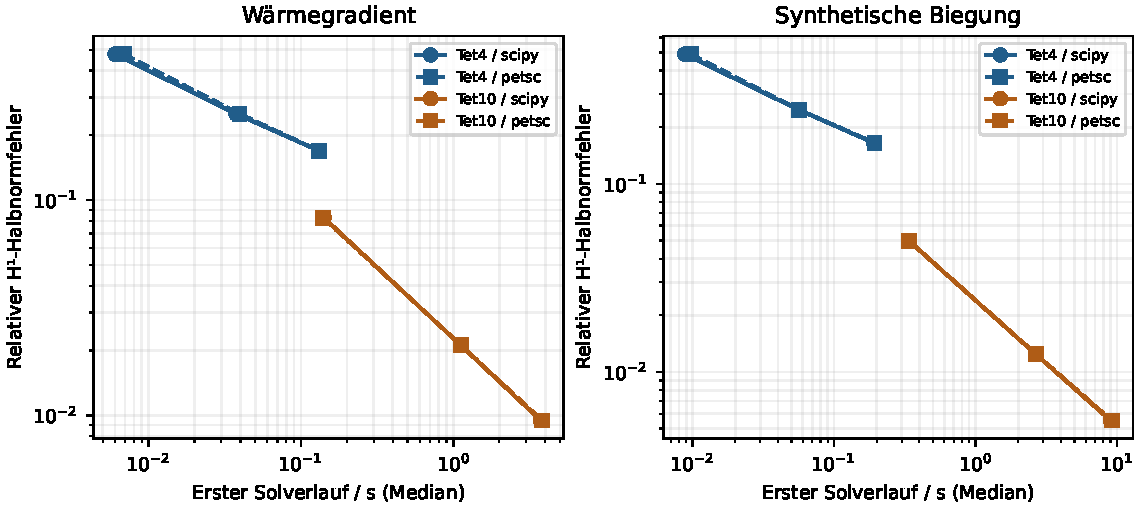
\includegraphics[width=\textwidth]{assets/verification-accuracy-cost.pdf}
\caption{Historische Genauigkeit gegen gemessene Erstlaufzeit. Linien verbinden
die drei tatsächlich gemessenen Netze; sie sind keine Interpolation oder
Leistungsprognose. Eigene Abbildung aus dem versionierten M7-Bestand.}
\label{vv:cost}
\end{figure}

\section{Positive und negative Befunde}
Die vorab gewählten relativen Genauigkeitsziele sind 0.5, 0.25 und 0.125.
Kostenbudgets sind 1, 5 und 20 s bei maximal 512 MiB RSS. Es wird aus den
gemessenen Kandidaten gewählt; kein fehlender größerer Tet4-Lauf wird geschätzt.
Backendparität wird mit $\mathrm{rtol}=10^{-8}$ und absoluten Toleranzen
$10^{-10}$ K bzw. $10^{-11}$ m geprüft. Residuen und Bilanzen müssen unter
$10^{-9}$ in den jeweiligen SI-Einheiten liegen.

Tet4 ist für die groben Ziele 0.5 und 0.25 in diesem Bestand schneller.
Das Ziel 0.125 erreicht Tet4 bis $N=6$ in beiden Fällen und mit beiden Backends
nicht: vier Auswahlen bleiben ausdrücklich \texttt{null}. Dafür wird kein
Geschwindigkeitsverhältnis berechnet. Tet10 erzielt in den vorgegebenen
Kostenbudgets kleinere Fehler. Ein ungemessener größerer Tet4-Lauf könnte die
Abwägung verändern. PETSc zeigt hier keinen allgemeinen Zeitvorteil und einen
höheren Prozess-RSS.

Die Streuung aus drei Wiederholungen beschreibt lediglich diesen Messbestand.
Hardware, Containerlimits, BLAS, Solveroptionen und Problemstruktur beeinflussen
die Übertragbarkeit. Die Budgets sind Auswahlregeln für den Vergleich und keine
zeitabhängigen CI-Abnahmeschranken. Die Abbildung begründet keine
Skalierungsbehauptung für große oder verteilte Rechnungen.
